\chapter{\glsentrylong{JPEG}}

\section{\glsentrylong{ITU} international standard}
\begin{itemize}
\item Developed by the
  \href{https://www.itu.int}{ITU}, \gls{JPEG}
  \cite{ccitt.t81} is
  supported by all Web browsers, and most image viewers.
\end{itemize}
\vspace{-2ex}
\begin{center}
  \href{https://en.wikipedia.org/wiki/Magnetic_resonance_imaging_of_the_brain#/media/File:MRI_of_Human_Brain.jpg}{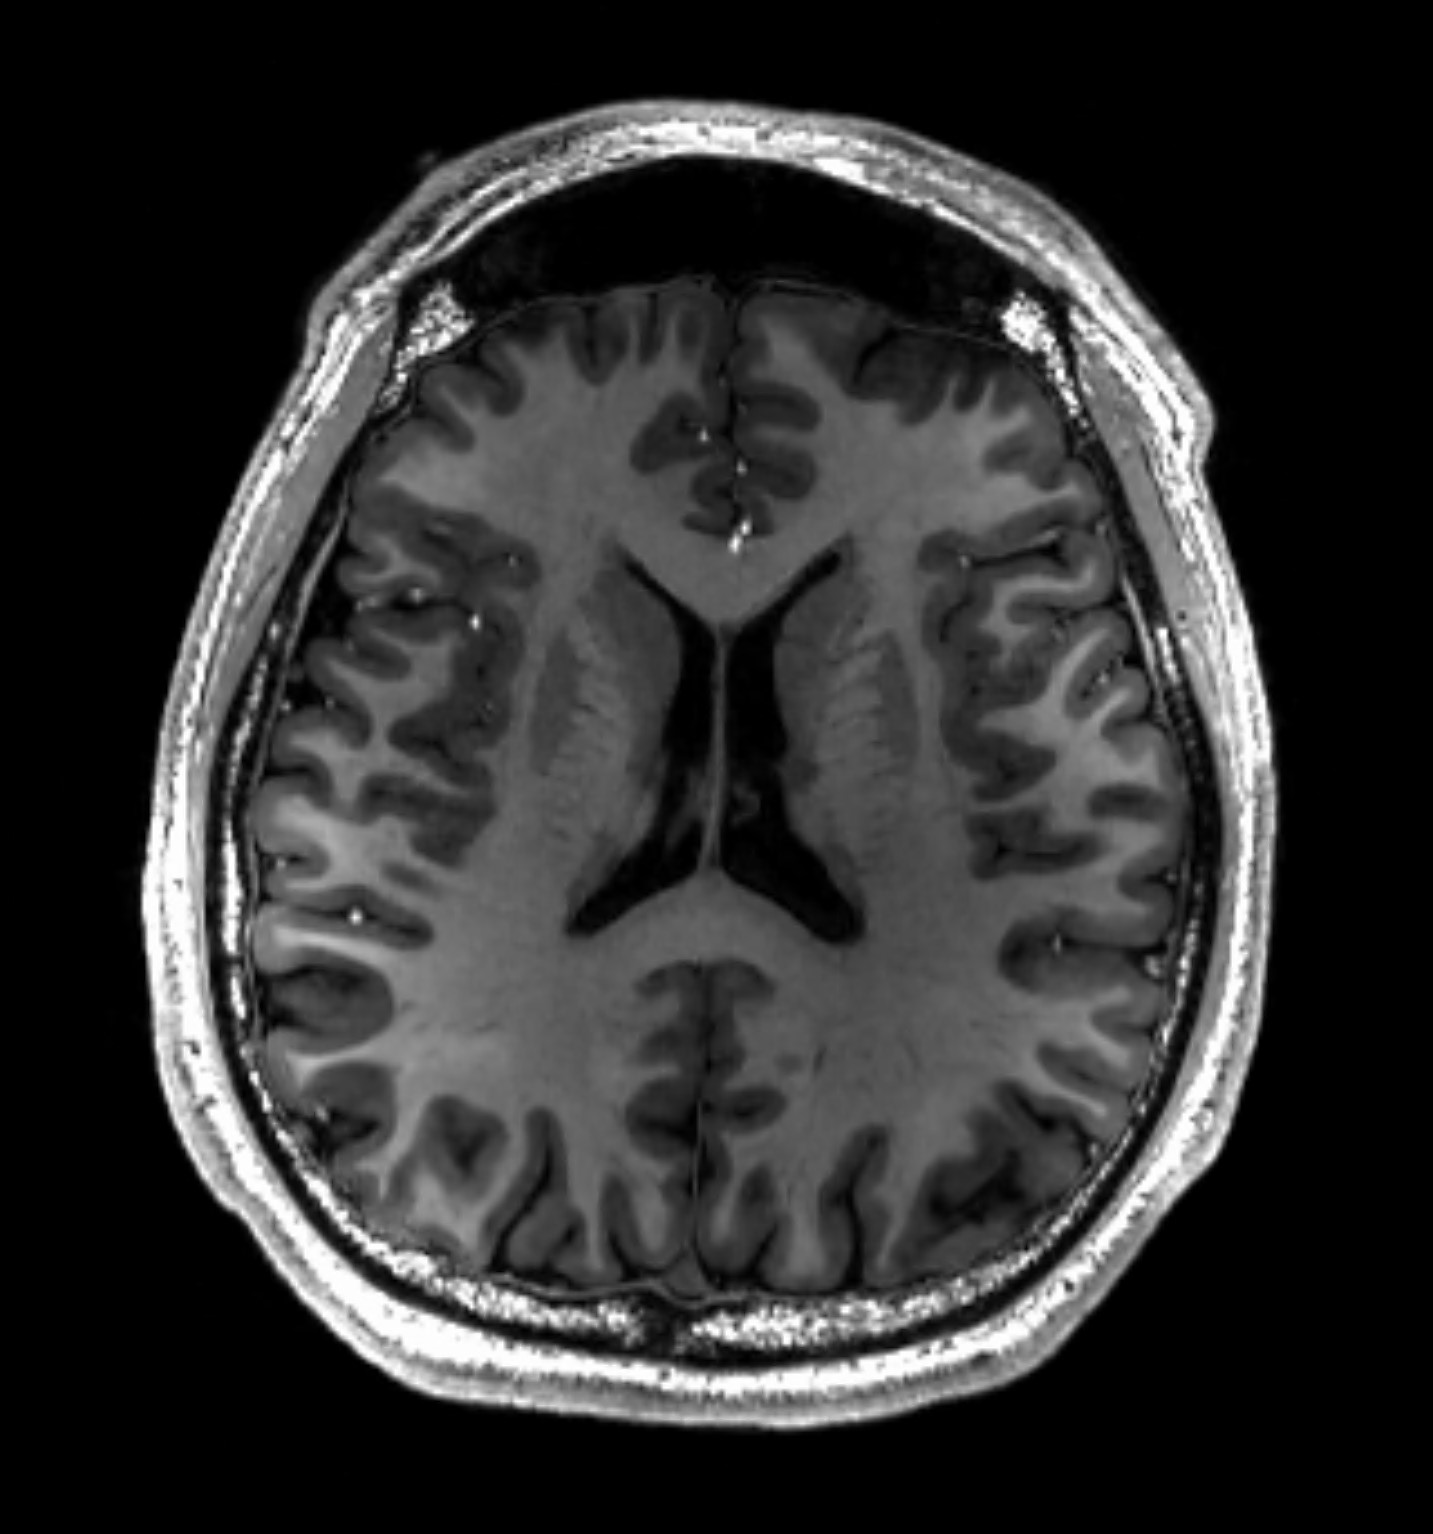
\includegraphics[width=4.0cm]{MRI_of_Human_Brain}}\\
  (click on the image)
\end{center}

\section{Lossy compression of color natural images}
\begin{itemize}
\item Designed for achieve high compression ratios, but at the expense of reducing quality.
  \item Raster images with up to ($2^{16}-1$)x($2^{16}-1$) pixels.
\item Pixels must be gray-scale or \gls{RGB}, 8 bits/channel.
\end{itemize}
\vspace{-2ex}
\begin{center}
  \href{https://www.thewebmaster.com/jpeg-definitive-guide/}{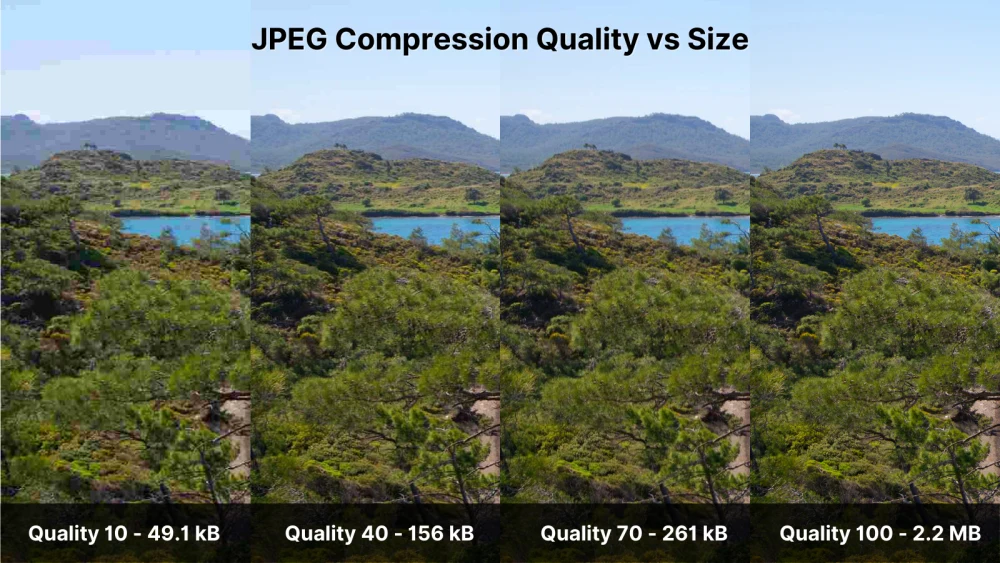
\includegraphics[width=8.5cm]{JPEG_Quality_vs_Size}}
\end{center}

\section{Algorithm (1/2)}
\begin{enumerate}
\item Convert from the \gls{RGB} color space to the \gls{YCrCb} color
  space. Only if the input image is in color.
\item Subsample the crominance (Cr and Cb channels). /* Lossy step */
\item Divide each channel in blocks of size 8x8.
\item Transform each block using the \gls{DCT}.
\item Quantize the \gls{DCT} coefficients. /* Lossy step */
\item Entropy encode the quantized coefficients.
\end{enumerate}

\section*{Algorithm (2/2)}
\begin{itemize}
\item A graphic description of a compression of a gray-scale image.
\end{itemize}
\vspace{-2ex}
\begin{center}
  \href{https://link.springer.com/article/10.1007/s40799-019-00358-4}{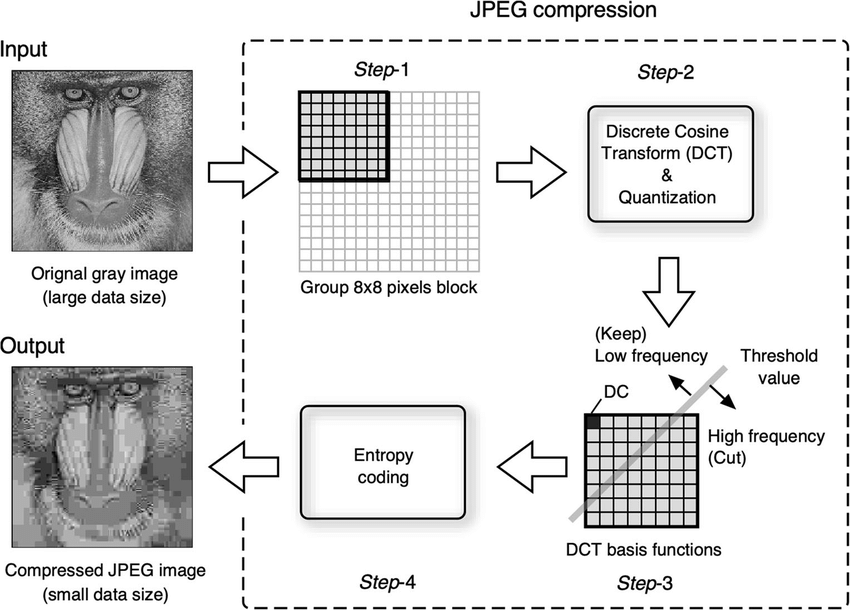
\includegraphics[width=8.5cm]{JPEG}}
\end{center}

\section{Artifacts}
\begin{itemize}
\item The human eye is sensitive to the 8x8-blockiness.
\end{itemize}
\vspace{-2ex}
\begin{center}
  \href{https://thesai.org/Publications/ViewPaper?Volume=6&Issue=4&Code=ijacsa&SerialNo=16}{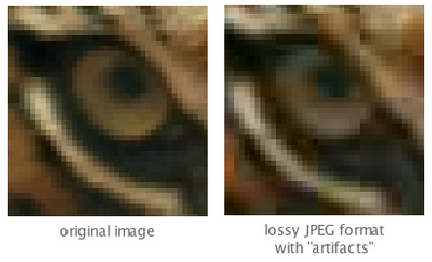
\includegraphics[width=10cm]{JPEG_blocking}}
\end{center}

\section{Progressive rendering}
\begin{itemize}
\item Optinal. Blocks are reconstructed coefficient-by-coefficient following the Zig-Zag ordering.
\item During a progressive visualization, blocks display higher
  spatial frequencies.
\end{itemize}
\begin{center}
  \href{https://es.m.wikipedia.org/wiki/Archivo:Zigzag_scanning.jpg}{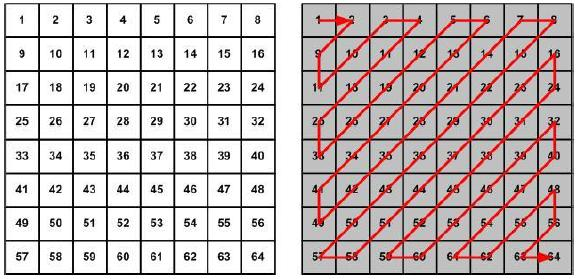
\includegraphics[width=8cm]{Zigzag_scanning}}
\end{center}

\section{Image metadata}